\documentclass[msthesis.tex]{subfiles}

\begin{document}
\chapter{Results}
In this section, the quantitative and visualization results from the methods presented in the chapter \ref{chap:methods} will be presented. The first two sections will present results from preprocessing of the DWI images mentioned in \autoref{sec:connectome_generation} and subsequent connectivity matrices. The next sections will set to statistically describe the nature of the data as well as classification results based on the comprehensive classification parameters explained in \autoref{tab:classify_combo}.

\section{Preprocessing Visualization}
\begin{figure}
    \centering
    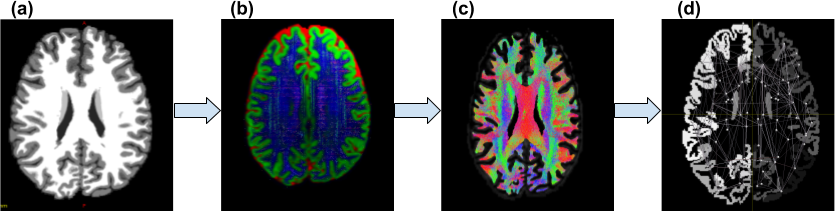
\includegraphics[width=\textwidth]{images/Preprocessing_pipeline.png}
    %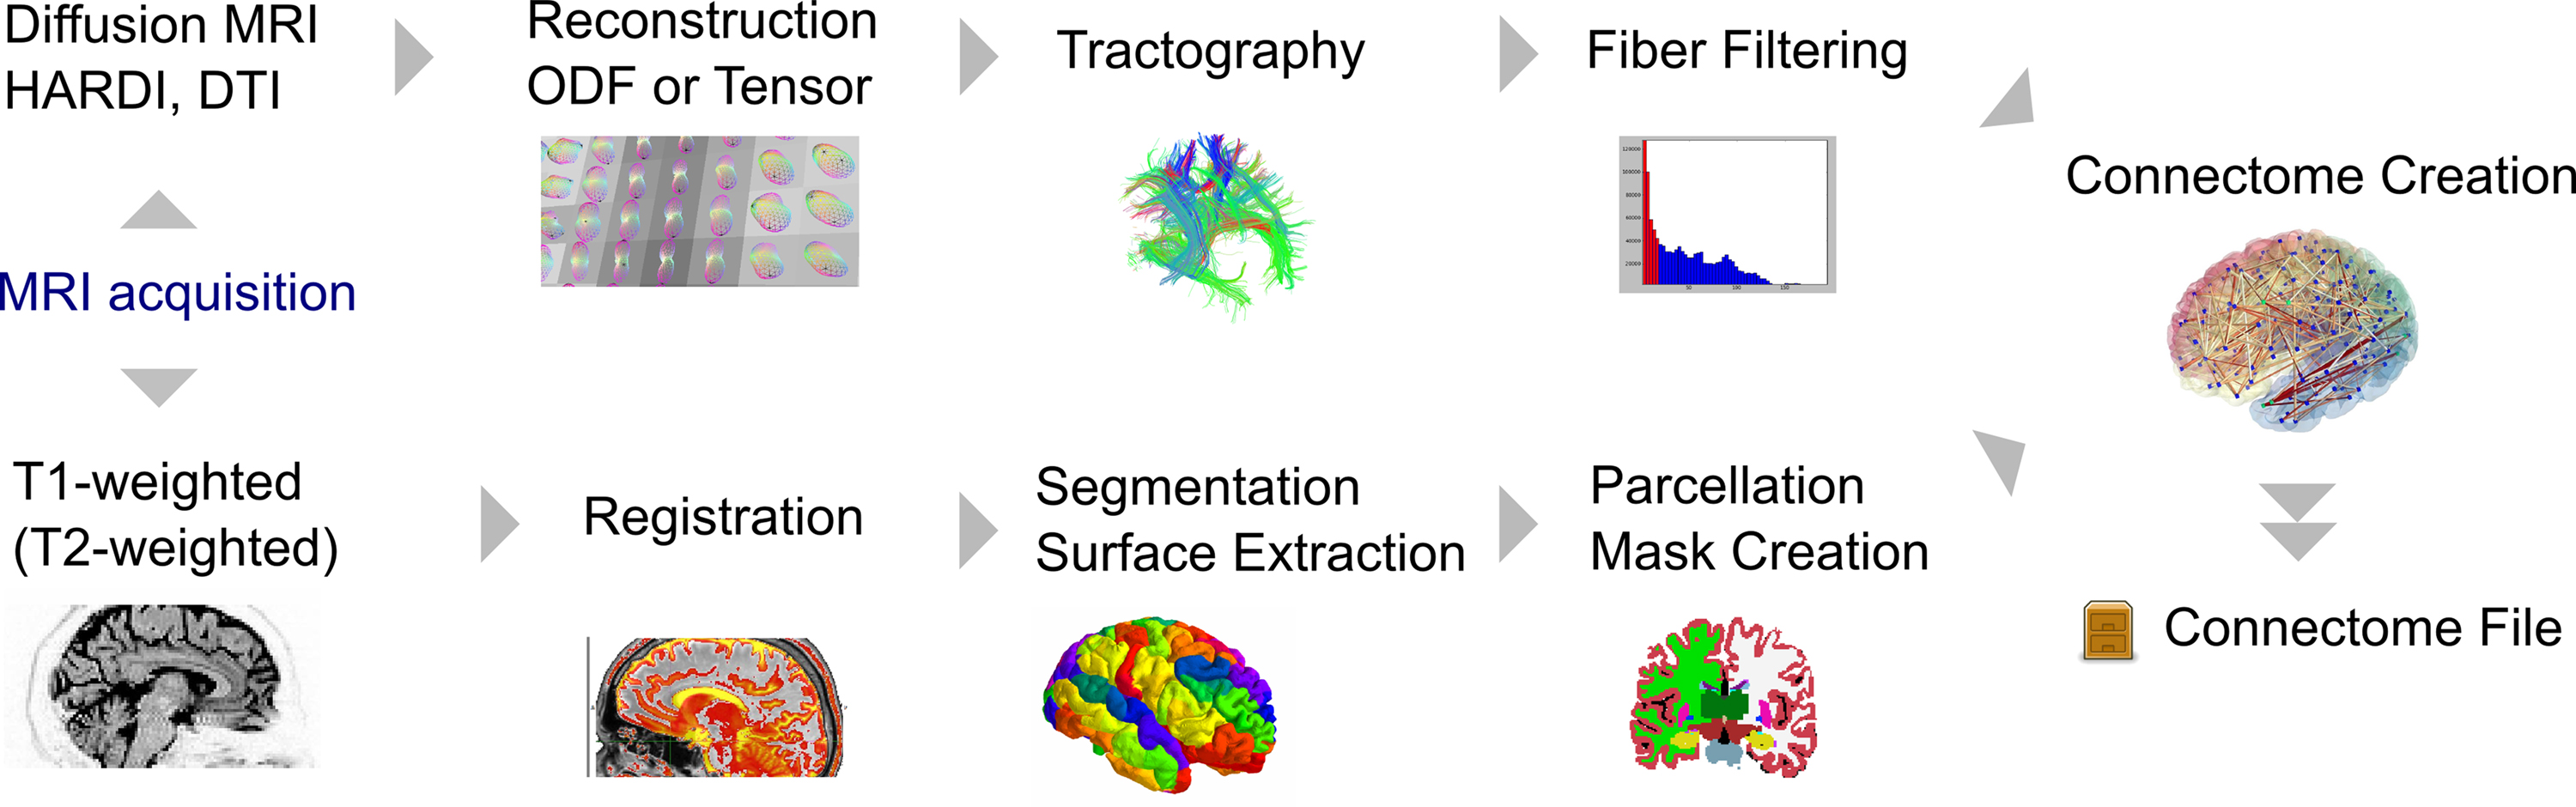
\includegraphics[width=\textwidth]{images/connectome_creation_workflow.png}
    %\cite{gerhard2011connectome}
    \caption{Visualization of pipeline used to create a connectome for each subject (a) Five tissue segmented image visualized in grayscale. (b) A slice of a 4D image mapped in 3D using RGB encoding tissue densities, CSF as red, GM as green and WM as blue. (c) Fiber tractography of one million fibers produced using probabilistic tractography overlaid on an axial slice of the brain. (d) The nodes of the connectome representing ROIs overlaid on an axial slice}
    \label{fig:preproc}
\end{figure}

During the process of generating the connectome (\autoref{subsec:connectomegeneration}) visual inspection was required to understand and investigate the properties of different types of images produced. The following results were obtained and anlayzed for adherence to conceptual the framework in \autoref{sec:creating_connectome}. 

The 5TT image obtained was 4D and could not be easily displayed in 3D. In \autoref{fig:preproc}.a the 4D image is displayed according to the grayscale mapping in 3D. It was observed that the 5TT images did not contain any errorneous labels. In this 4D image, each volume represents the corresponding tissue densities of WM, GM and CSF. The 4D image is then visualized as an RGB image with each volume getting its specific color (\autoref{fig:preproc}.b). With the help of the RGB image the alignment of the fODFs seemed plausible on zooming.

Further, the one million fibers tractography was obtained with correspondence to the color coding of the fibers that run along the x,y and z axes respectively. The nodes of the connectome were then represented by the center of mass in the parcellated regions, the intensity of the image does not represent signal intensity but different parcels. 


\section{Connectome Visualization}
\label{sec:connectome_generation}
\begin{figure}
    \centering
    %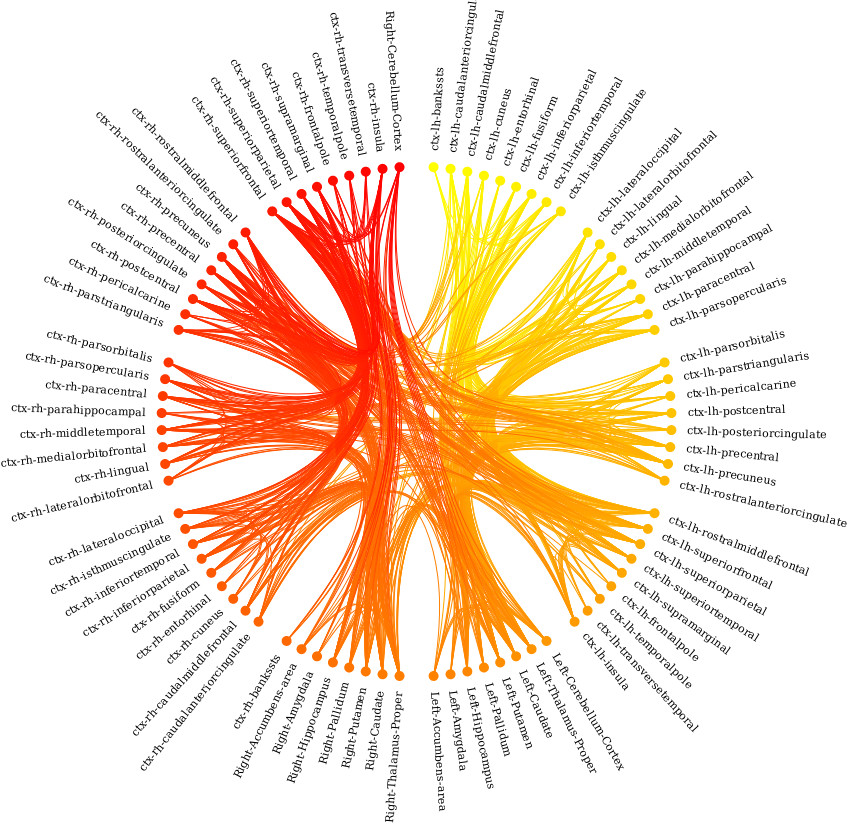
\includegraphics[width=\textwidth]{images/brain-data-viewer_2.png}
    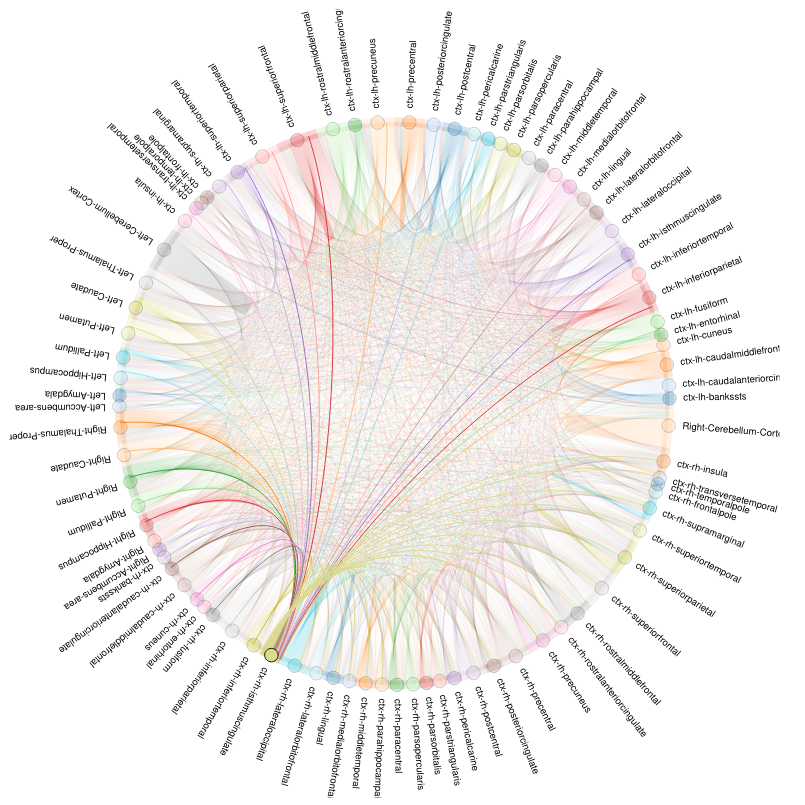
\includegraphics[width=\textwidth]{images/bokeh_plot_allsubjects.png}
    \caption{A chord plot representing the group averaged connectome for all subjects. The number of arcs (edges) represent the number of streamlines between any two ROIS. The ROIs are represented as the nodes in the diagram at the end of the circle. They are labelled according to the Desikan Killiany Atlas. The presence of multiple arcs get bundled together and increased multiple arcs are represented by one arc with higher thickness. In this interactive visualization, the cortical region isthmus cingulate is selected as the source node and the all the edges convergent on this node are colored according to the terminal node.}
    \label{fig:connectome_num_streamlines}
\end{figure}

In the chord plot represented in \autoref{fig:connectome_num_streamlines} the cortical region isthmus cingulate in the right hemisphere is selected. Its has prominent connections to the cortical regions inferior parietal, superior frontal, superior temporal in the left hemisphere. It is also connected to the subcortical regions Hippocampus, Putamen and thalamus proper in the right hemisphere. A set of weak connections to the cortical region fusiform is also well represented by this diagram. This interactive visualization helped determine the connections between brain regions. 


\section{Feature Analysis}
From the preprocessing pipeline presented in \autoref{sec:connectome_generation} there were three types of features obtained for each subject. The number of streamlines, the mean streamline length and the mean FA. Each of these features encodes a different biological property of between ROI connections and could hold different results for the classification. There is no current consensus on which feature qualifies as an effective measure of 'connectivity' between any two nodes (\cite{yeh2020mapping}). Hence, it was required to determine which one of them is actually more interpretable as well as best performing for a generic implementation independent of the target label. Further, exclusion of self loops has also been experimentally justified to not provide any added benefit to classification accuracy. 
\subsection{Differences in connectivity metric}
\begin{figure}
    \centering
    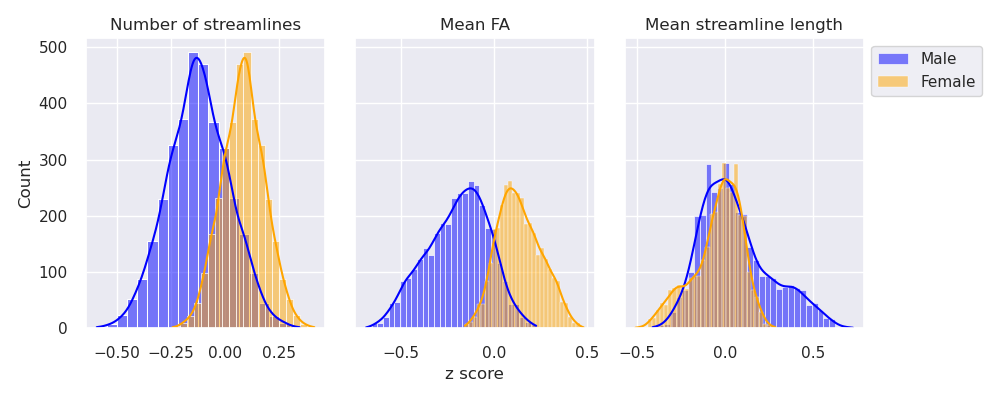
\includegraphics[width=\textwidth]{images/zscoredist.png}
    \caption{Histograms representing the frequency of mean z scores for different types of features.}
    \label{fig:hist_zscores}
\end{figure} 
As mentioned above, it was important to explore different types of connectivity metrics obtained from the connectivity matrices constructed using methodology \autoref{fig:hist_zscores}. The three types of metrics were the mean FA, mean streamline length and number of streamlines. The number of streamlines and the mean streamline length could have contained biases as they were constructed in the individual subject's space and hence comparing these numerical values for any two subjects did not seem a logically intuitive, but due to the informed filtering using the SIFT algorithm, these biases were well corrected for an these measure could be compared (\cite{yeh2020mapping}). 

A histogram for the three different feature or connectivity types could help speculate which one performs better while classifying target variables.  Using Standard scalar each feature was standardized by removing the mean and scaling it to unit variance. After scaling the feature value for each subject is represented by a z statistic. The mean of the z statistic (of one feature) for all training subjects was then taken to form a histogram on the type of feature. So for each connectivity metric there are 3486 features.

The distribution for the number of streamlines for males and females in the training data are both non-overlapping and well-normally distributed. This could contribute towards the good performance of classifiers when training on the basis of number of streamlines. Further on the basis of informed filtering of the fiber tracts, it is plausibe tha t

The plot for the number of streamlines on the left shows that women have comparatively higher z scores as compared to men. This means that women have on an average more number of streamlines in the same between ROI connection. 

The Mean FA feature for women is also showing higher Z score which means that women have higher mean FA as compared to the average when considering a mixture of males and females as the training set. 

On the other hand, an opposite trend is seen in the case of mean streamline length. Women have lower z scores as compared to men, this means that they have shorter streamline lengths. Which seems plausible because generally the size of the brain in women is smaller. 

\subsection{Self loops}
\label{res:selfloops}

The results for the experiment mentioned in section \ref{sec:exclusion} are presented in table \ref{table:selfloops}. For the independent test data all p-values are $p>0.05$ and the t statistic values represent the differences in the classification metrics with and without the inclusion of self loops. The low absolute values of the t-statistic further increased the evidence for insignificance of inclusion of self loops for classification accuracy.

\begin{table}
\label{table:selfloops_combined}
\csvreader[
  tabular=|p{0.13\textwidth}|p{0.15\textwidth}|p{0.29\textwidth}|p{0.08\textwidth}|p{0.09\textwidth}|,
  table head= \specialrule{0.2em}{0.05em}{0.05em} Target Label & Metric & Feature & T test & P value\\ \hline,
  late after last line=\\\hline,
]{tables/Combined_self_loops.csv}{}%
{\csvcoli  & \csvcoliii & \csvcoliv & \csvcolv & \csvcolvi}
\caption{Results for a paired samples t-test carried where paired samples are the classification metrics of the data with and without the inclusion of self loops. The corresponding p values are for two arrays for the same classification metric with each array representing classification metric for the five different personality traits. Based on test data only.}
\end{table}

\section{Baseline analysis}
\begin{figure}
    \centering
    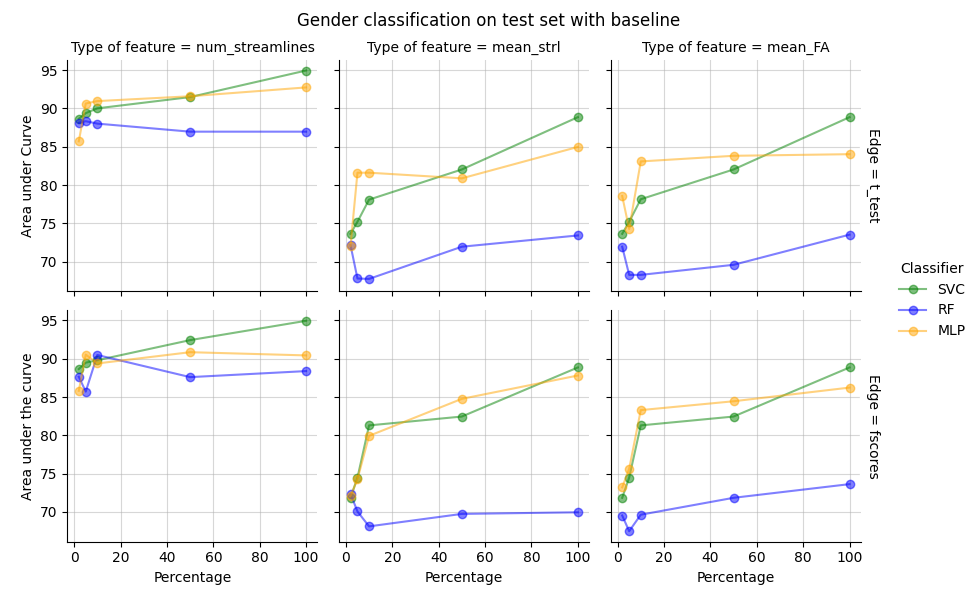
\includegraphics[width=\textwidth]{images/baseline_results_gender.png}
    \caption{Baseline analysis for gender classification. The area under the curve represented as a function of percentage of features. }
    \label{fig:my_label}
\end{figure}
\begin{figure}
    \centering
    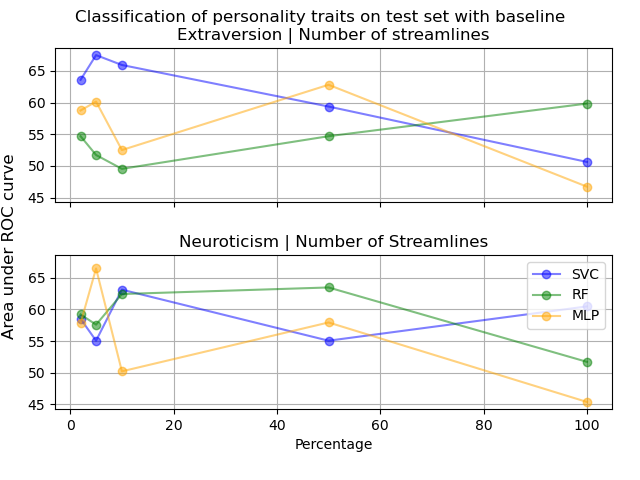
\includegraphics[width=0.8\textwidth]{images/persona_2.png}
    \caption{Baseline analysis on the basis of personality traits using pearson correlation coefficient. In a general trend it can be seen that doing some feature selection is beneficial for the classification.}
    \label{fig:persona base}
\end{figure}
In the baseline analysis choosing the number of streamlines with any type filter methods still retains most of the classification information. There is not much reduction in the AUC from using all the features until retaining only a small subset of features.

For both the personality traits and the gender based classification, feature selection seems profitable in terms of going towards interpretability. For the personality based classification which is a tough task doing this was difficult and hence....

\subsection{Solver}
After filtering according to the edges being selected only when there is at least one streamline per subject. On the basis of the training subjects, the number of features for which all the subjects have a at least one streamline with them is 1150. The input graph is hence formed on the basis of this with this number determining the upper bound of the number of edges in our input graph. 

In Fig. \ref{fig:gender_num_strls_10} the MEWS solver based implementation reduces the input graph based on the fscores to infer the most important set of connections. In this graph the edges obtained from Fig. \ref{fig:solver_based_gender_10} were traced back to the original \textit{dataframe} containing the data about number of streamlines for all subjects. The number of streamlines between the regions delineated were determined to put together in the chord graph. From the thickness of the arcs in the chord graph the Left-Palladium and right thalamus proper seem to have the maximum number of connections between them. Further, the subcortical regions seem to have more number of streamlines between them than the cortical regions. 


\begin{figure}
    \centering
    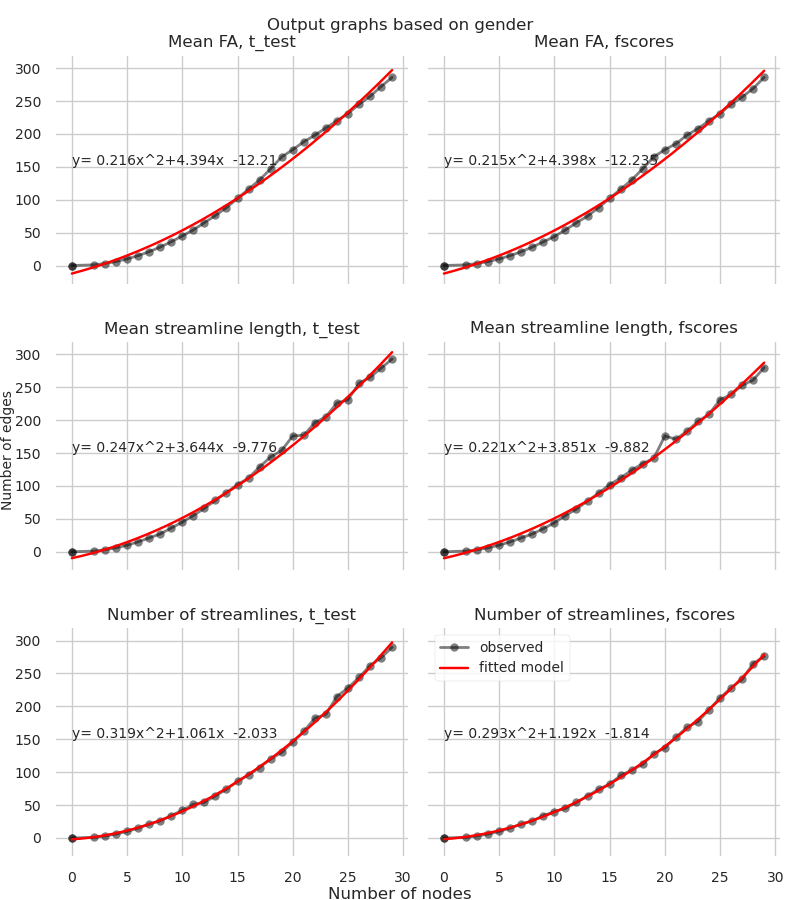
\includegraphics[width=0.8\textwidth]{images/Gender_nodes_preserved.png}
    \caption{Edges preserved as a function of nodes in the case of gender subgraph reduction}
    \label{fig:fun_num_edges}
\end{figure}

\iffalse
\begin{figure}
    \centering
    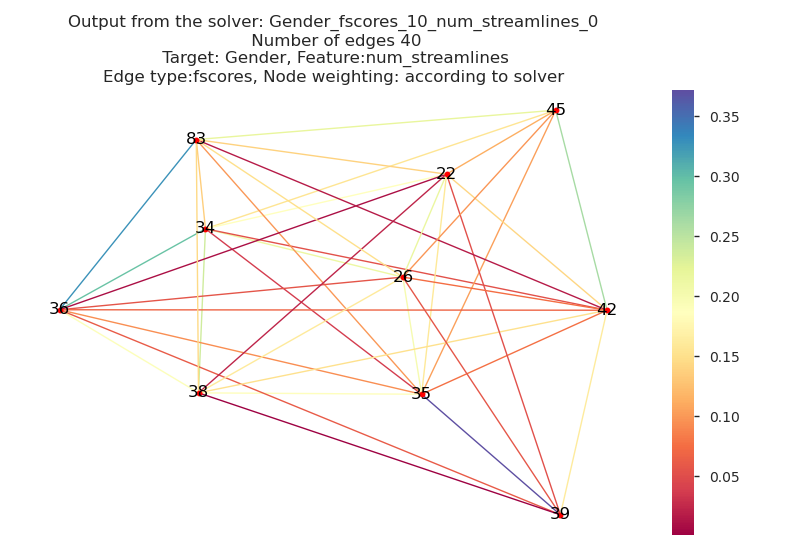
\includegraphics[width=0.5\textwidth]{images/gender10nodes.png}
    \caption{Caption}
    \label{fig:solver_based_gender_10}
\end{figure}

\fi

\begin{figure}
    \centering
    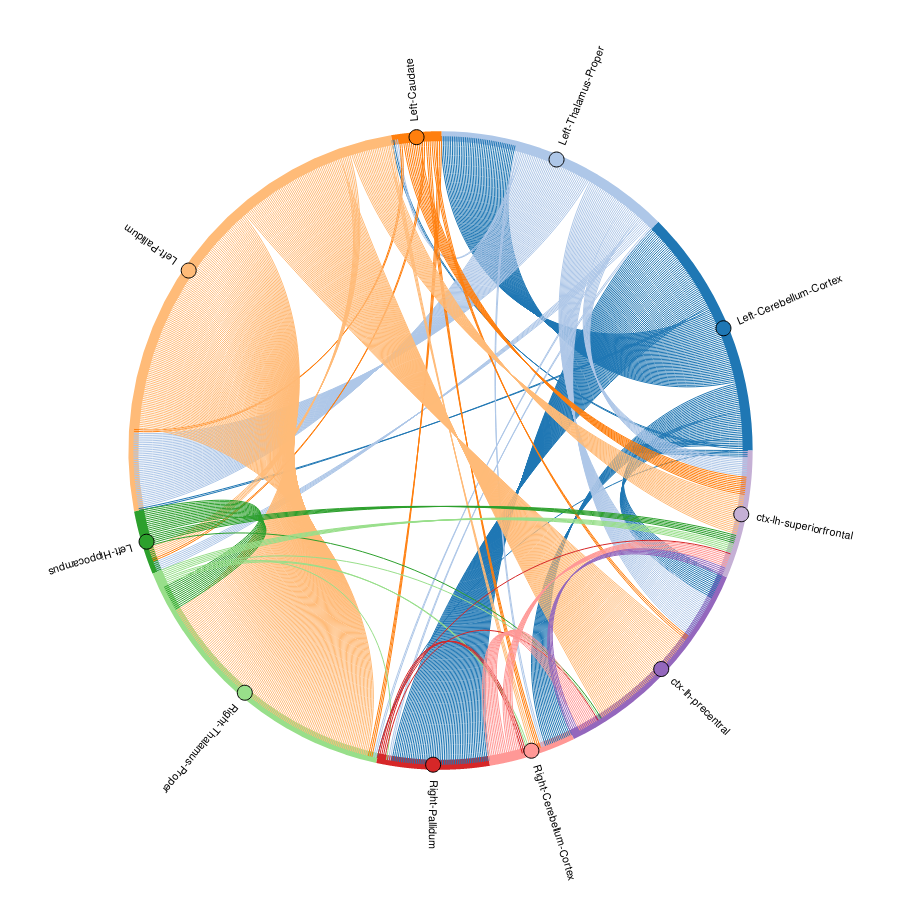
\includegraphics[width=0.9\textwidth]{images/gender10nodes_numstrls.png}
    \caption{10 most important nodes determined using the solver based analysis using the fscores for the Gender based classification. This graph is a Chord graph implemented using Holoviews (\cite{stevens2015holoviews}). The number of edges between any two nodes represent the number of streamlines between them. The fscores were used in order to determine the importance of the connections, the filtered edges retraced back to the original matrix yielded this result. The number of streamlines was averaged for all subjects and then the filtered edges based on the solver were produced. Multiple edges are drawn in the chord type graph where the number of edges represents the number of streamlines.}
    \label{fig:gender_num_strls_10}
\end{figure}


For the features determined by the subgraph. The reduced features were put through an independent samples t-test for gender differences. 

\iffalse
\begin{table}
\label{table:10strls_gender}
\csvreader[
  tabular=|c*{4}{|c}|,
  table head= \hline feature & ROI & ROI & P value\\ \hline,
  late after last line=\\\hline,
]{tables/gender10_numstrls.csv}{}%
{\csvcoli & \csvcolii & \csvcoliii & \csvcoliv }
\caption{Results for an independent samples t-test carried, The corresponding p values are for the different number of streamlines for males and femalestvod .}
\end{table}
\fi


\iffalse
\begin{figure}
    \centering
    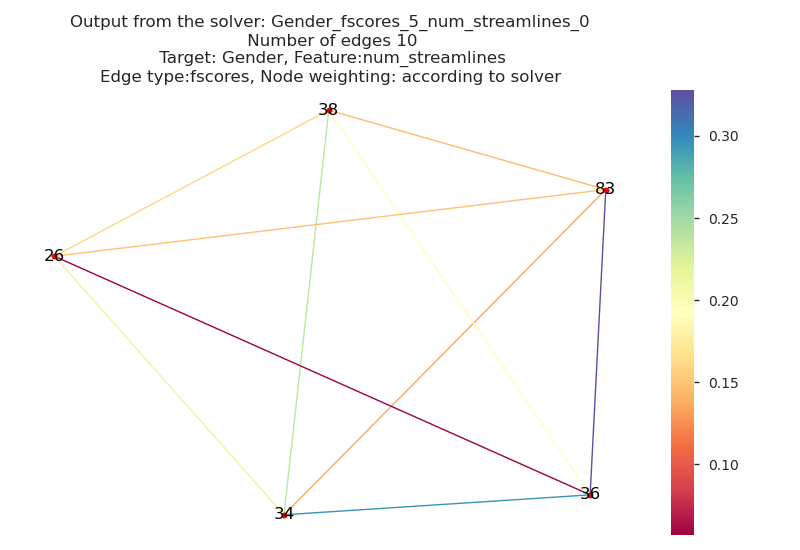
\includegraphics[width=0.8\textwidth]{images/Gender5nodes.png}
    \caption{Caption}
    \label{fig:}
\end{figure}

\begin{figure}
    \centering
    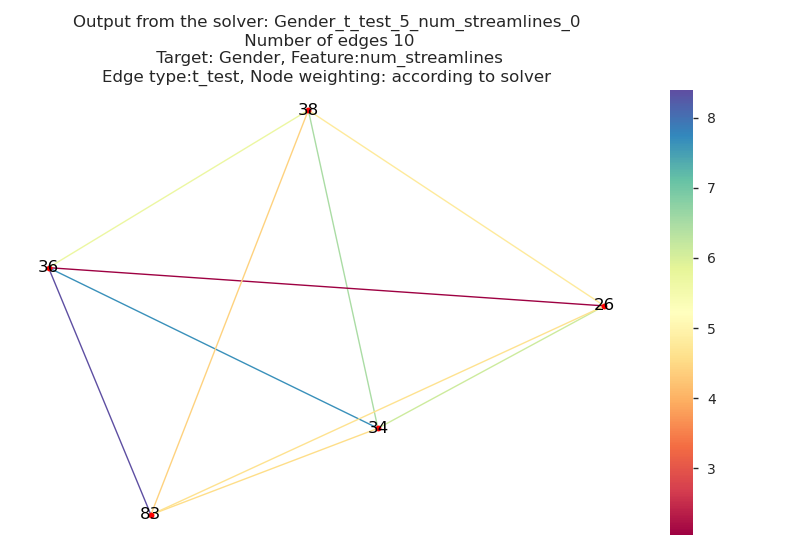
\includegraphics{images/Gender5nodes_test.png}
    \caption{Caption}
    \label{fig:my_label}
\end{figure}
\fi
\iffalse
\section{Solver and baseline comparison}
\begin{figure}
    \centering
    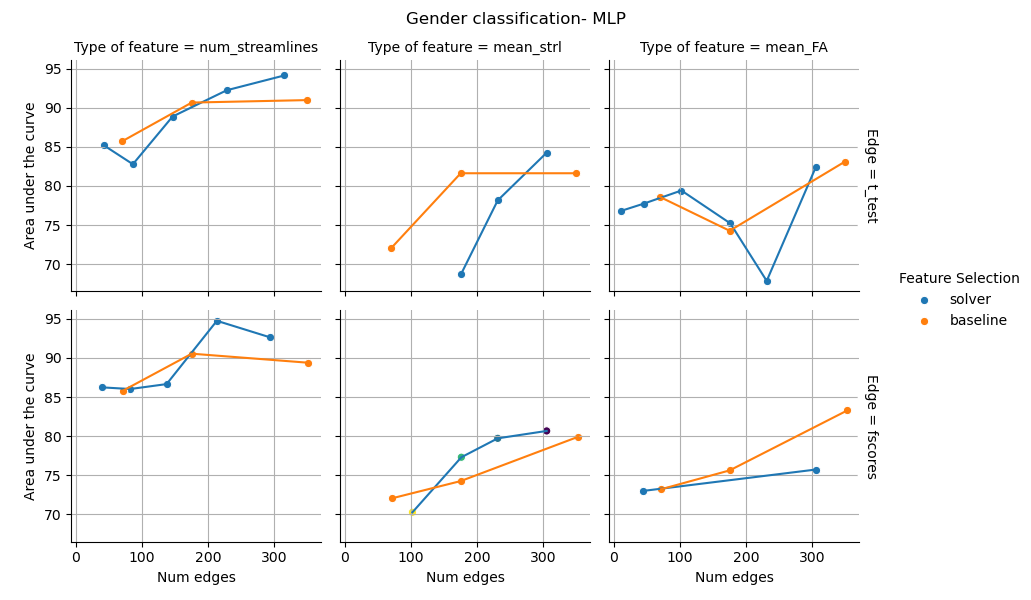
\includegraphics[width = \textwidth]{images/comparison_roc_auc_MLP.png}
    \caption{Caption}
    \label{fig:mlpgender}
\end{figure}
\begin{figure}
    \centering
    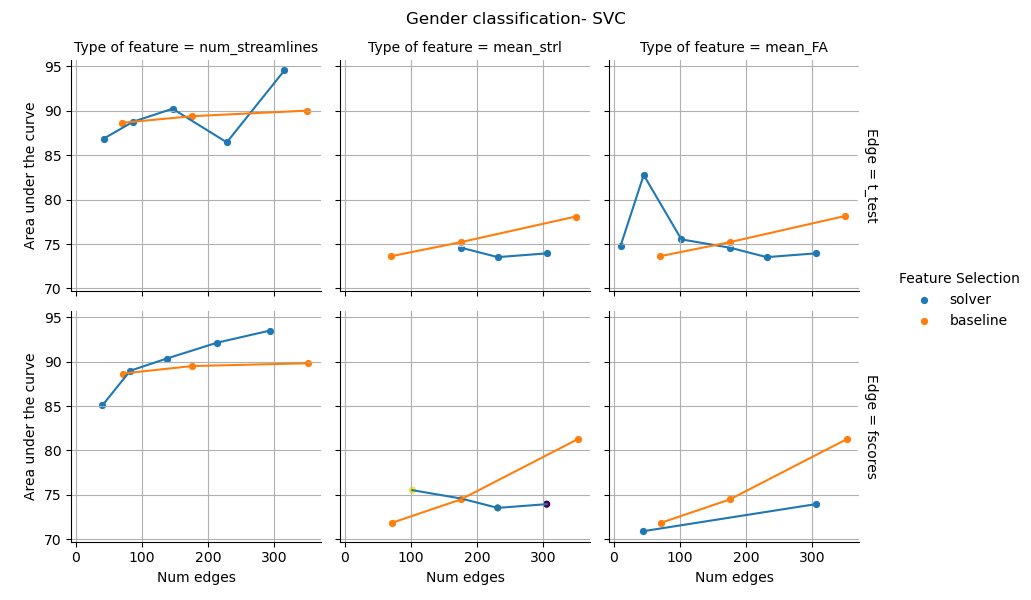
\includegraphics[width = \textwidth]{images/comparison_roc_auc_SVC.png}
    \caption{Caption}
    \label{fig:svcgender}
\end{figure}

\begin{figure}
    \centering
    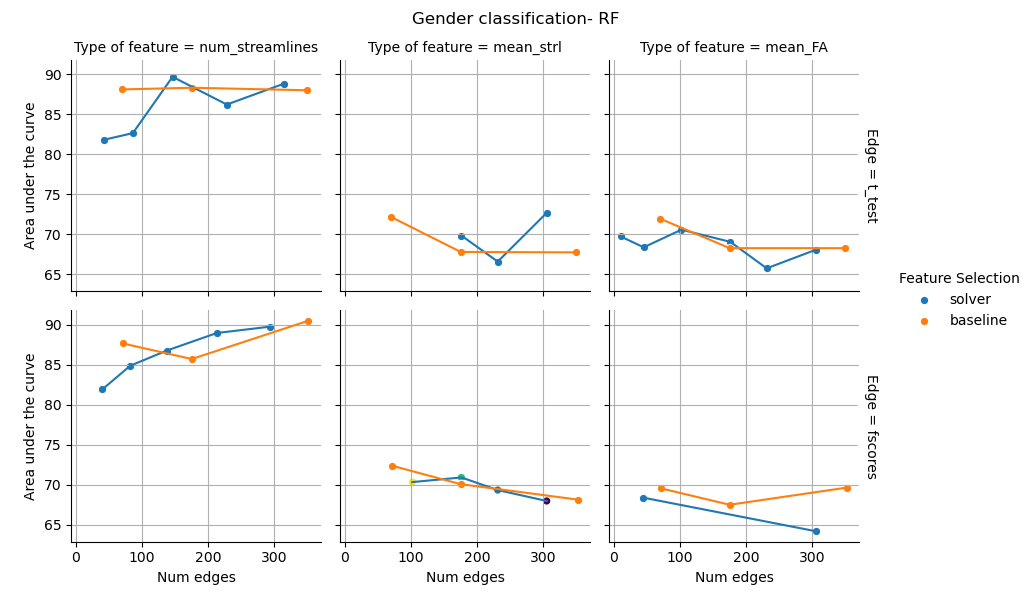
\includegraphics[width = \textwidth]{images/comparison_roc_auc_RF.png}
    \caption{Caption}
    \label{fig:rfgender}
\end{figure}
\fi





Judging on the basis of the area under the curve for gender based classification, it is best to compare feature wise.

Consider the mean FA feature first, for this feature the solver based approach does better than or equivalently well as the baseline when the number of edges preserved is small. This is not surprising since the number of edges preserved is a function of the number of nodes specified by the solver based technique. When a specified number of edges would be wanted to be preserved then the features corresponding to only those nodes will be preserved, this makes an inherent bias into which features will be preserved by the solver. Since all one node might have multiple highly relevant performance features but we want to preserve a given number of nodes, so the other less performing feature might be selected since a particular node has to be selected.



\section{Classification}

\begin{figure}
    \centering
    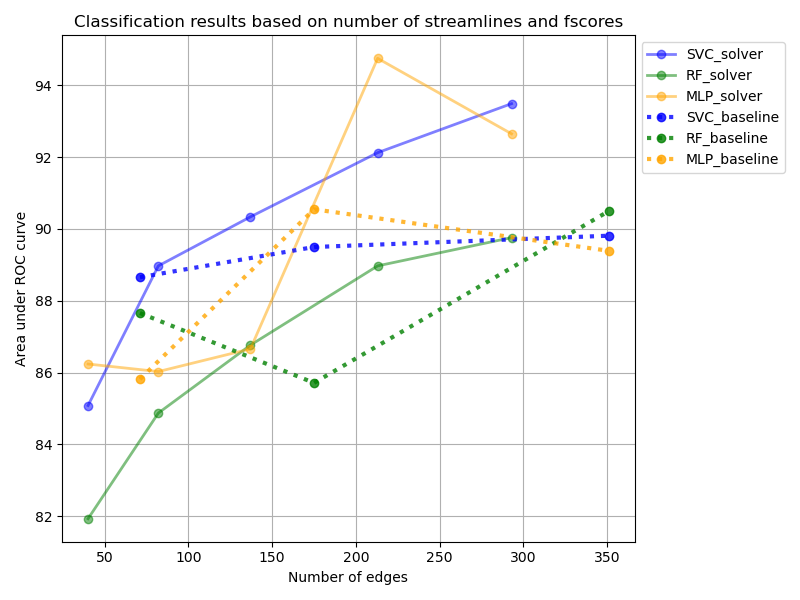
\includegraphics[width=0.8\textwidth]{images/select_clf_auc_gender.png}
    \caption{Comparison of area under the ROC curve for gender classification on the independent test set. The performance of three classifiers Support Vector Machines, Random Forest and Multilayer perceptron on the basis of features filtered according to the solver and baseline experiments respectively.}
    \label{fig:clf_solver results}
\end{figure}

\begin{figure}
    \centering
    %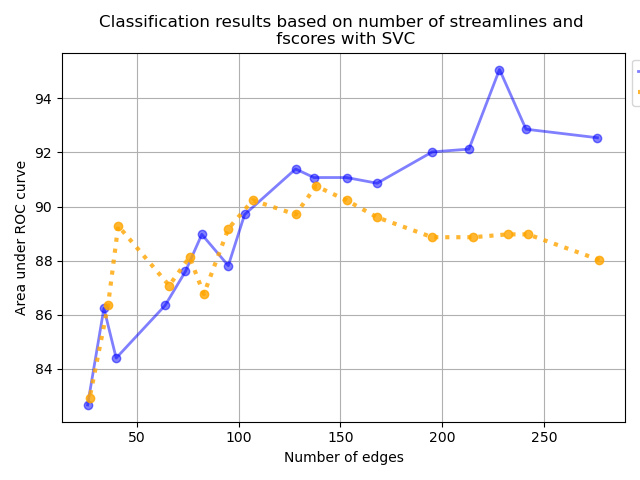
\includegraphics[width=0.8\textwidth]{images/select_clf_auc_gender_2_svc.png}
    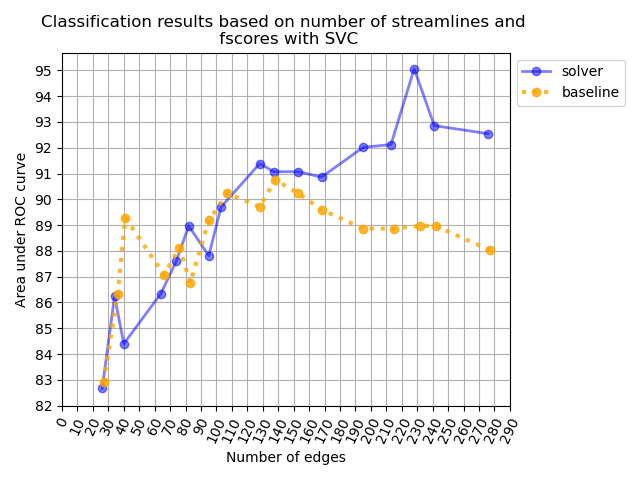
\includegraphics[width=0.8\textwidth]{images/select_clf_auf_gender_2_scaled.png}
    \caption{Classification using solver and baseline for the exact same number of features selected in each case.}
    \label{fig:svcgender}
\end{figure}

On closely analyzing the behaviour from the curve as viewed above. The SVM based classification produced more stable results. More data points were then sampled. This time the number of edges preserved by the solver was used to decide the parameter top $k$ percentile of features to be preserved in the baseline analysis. From the \autoref{fig:svcgender}, it became clear that after a cutoff number of edges, i.e. precisely 137 (obtained from the function in \autoref{fig:fun_num_edges} and the preprocessed files, the solver definitely does better than the baseline analysis. Even for the number of edges below 137, the results remain comparable but more interpretable. So for the solver, the number of nodes for gender classification that definitely yields better results than the baseline experiments after 137 edges. Corresponds to 20 nodes i.e. ($137 \approx 0.285* 400 + 1.467(20) - 3.888 = 114 + 29.34-3.88 = 139.46$). So for below 20 nodes there is a bit of a compromise for classifier performance but increased interpretability and ease of visualization. While for higher than 20 nodes, there is a decrease in interpretability but an increase in classifier performance.

\subsection{Best parameters}
For our configuration using Multilayer perceptron for the solver based reduction, classification of gender using the feature selection technique of fscores and refit metric balanced accuracy. Baseline based on 5\% of features. The parameters for the best estimator of the cross validation turn out to be the same, this justifies that the solver based method works better than the baseline method when it comes to classification accuracy and also leads to an increase in the interpretability.
% Best estimator {'solver': 'adam', 'learning_rate': 'adaptive', 'hidden_layer_sizes': (50, 100, 100, 50), 'alpha': 0.05, 'activation': 'relu'}
% ('MLP', 'Gender', 'random', 'fscores', 'baseline', 'num_streamlines', 5, 'balanced_accuracy', False)
%Bet estimator {'solver': 'adam', 'learning_rate': 'adaptive', 'hidden_layer_sizes': (50, 100, 100, 50), 'alpha': 0.05, 'activation': 'tanh'}
\begin{table}[b]
    \centering
    \begin{tabular}{|c|c|c|}
        \specialrule{0.1em}{0.05em}{0.05em}
        Hyperparameter & Solver & baseline \\
        \hline
        solver & adam & adam\\
        \hline
        hidden layer size &  50,100,100, 50 & 50,100,100,50\\
        \hline
        activation function & relu & tanh\\
        \hline
        alpha & 0.05 & 0.05\\
        \hline
        learning rate & adaptive & adaptive\\
        \hline
    \end{tabular}
    \caption{Cross validation parameters for MLP trained for gender classification. The parameters which give the best area under the curve for the use case mentioned in the section above have been presented}
    \label{tab:MLP best params}
\end{table}
The SVM seemed to give most stable results and the maximum area under the curve given by the for gender classification is 95\% for number of nodes 26. These parameters are for the solver based experiments and classifier SVC. For the best estimator with the baseline experiments the around 138 edges does the best with 91\% AUC so the parameters for that are presented in the table. 
%Best estimator {'C': 5.918565074193836, 'class_weight': 'balanced', 'gamma': 0.0004643818614121193, 'kernel': 'rbf'}
%Best estimator basline {'C': 0.5229762127721259, 'class_weight': None, 'gamma': 0.008523831363402392, 'kernel': 'rbf'}

\begin{table}[b]
    \centering
    \begin{tabular}{|c|c|c|}
        \specialrule{0.1em}{0.05em}{0.05em}
        Hyperparameter & Solver & baseline \\
        \hline
        C & 5.9 & 0.522\\
        \hline
        Gamma &  4e-4 &  8e-4\\
        \hline
        kernel &  rbf & rbf\\
        \hline
        class weight & balanced & None\\
        \hline
    \end{tabular}
    \caption{Cross validation parameters for SVC trained for gender classification. The parameters which give the best area under the curve for the use case mentioned in the section above have been presented}
    \label{tab:CSV best parameters}
\end{table}

\end{document}
